\documentclass[10pt]{beamer}
\usepackage[utf8]{inputenc}
\usepackage[czech]{babel}
\usepackage[abs]{overpic}
\usepackage{color}
\usepackage{tikz}

\usetheme[faculty=fi]{fibeamer}

\usepackage{color}

\definecolor{mygreen}{RGB}{51, 169, 54}

\title{Formal Biochemical Space for Specification and Analysis of Biochemical Processes} 
\subtitle{Obhajoba diplomovej práce}
\author[Matej Troják]{Matej Troják}

\newcommand{\header}{IV120: Úvod do problematiky a informace o kurzu}

\begin{document}

\frame{
\thispagestyle{empty}
\titlepage
}

% -------------------------------------------------------------

\frame{
\frametitle{Motivácia}

Časté problémy s modelmi:

\begin{itemize}
\item rekonštrukcia -- "spustiteľný" ~model
\item pochopenie -- aký systém model predstavuje?
\item interpretácia -- čo model vysvetľuje?
\end{itemize}

\begin{center}
\vspace*{-1.5cm}
\includegraphics[width=0.8\textwidth]{motivation}
\end{center}

}

% -------------------------------------------------------------

\frame{
\frametitle{Riešenie}

\textbf{Biochemical Space} (BCS) je doména biologických znalostí s formálnymi prvkami, ktorá poskytuje 

\begin{itemize}
\item popis,
\item anotáciu,
\item zdieľanie
\end{itemize}

špecificky zameraných biologických modelov.

\vspace{1cm}

\textbf{Motto}: \emph{formalizácia biologického popisu a anotácia modelov.}

}

% -------------------------------------------------------------

\frame{
\frametitle{Comprehensive Modelling Platform}

Webový framework pre integráciu biologických znalostí s výpočetnými modelmi a experimentami.

\begin{center}
\begin{columns}
\begin{column}{0.45\textwidth}

\begin{itemize}
	\item \url{e-photosynthesis.org}
\end{itemize}

\vspace{0.5cm}

\includegraphics[width=1\textwidth]{ephoto}

\end{column}

\begin{column}{0.45\textwidth}

\begin{itemize}
	\item \url{e-cyanobacterium.org}
\end{itemize}

\vspace{0.5cm}

\includegraphics[width=1\textwidth]{ecyano}

\end{column}
\end{columns}
\end{center}
}

% -------------------------------------------------------------

\frame{
\frametitle{BCS formát}
  
\begin{center}
 \hspace*{-0.7cm}\includegraphics[width=1.1\textwidth]{equation}
\end{center}

}

% -------------------------------------------------------------

\frame{
\frametitle{Prečo nový jazyk?}
 
Biochemical Space \textbf{Language} (BCSL)

\begin{itemize}

\item reprezentácia ľahko editovateľná a spravovateľná,

\item \emph{rule-based} -- zníženie náročnosti na pamäť a spracovanie,

\item čisto textový formát -- nie grafická reprezentácia,

\item priama interpretácia užívateľovi,

\item anotácia aj operačná sémantika pre analýzu.

\end{itemize}

}

% -------------------------------------------------------------

\frame{
\frametitle{Ako to funguje}
  
\begin{center}
 \hspace*{-0.7cm}\includegraphics[width=1.1\textwidth]{annot}
\end{center}

}

% -------------------------------------------------------------

\frame{
\frametitle{Výhody}

\begin{itemize}
\item model získa svoj biologický význam

\begin{itemize}
\item anotácia pre individuálne componenty/reakcie vždy ľahko dostupná
\item implementovaný model dostupný online
\end{itemize}

\item vymedzením vzťahu model ku BCS získame popis modelu v BCSL

\begin{itemize}
\item možnosť ďalšej analýzy
\item jednotná forma modelov -- porovnávanie
\end{itemize}

\end{itemize}

\begin{center}
\includegraphics[width=0.8\textwidth]{transformation}
\end{center}

}

% -------------------------------------------------------------

\frame{
\frametitle{Entity}
  
\includegraphics[width=1\textwidth]{hierarchy}

}

% -------------------------------------------------------------

\frame{
\frametitle{Abstrakcia komplexu}
  
\includegraphics[width=1\textwidth]{abstracton}

}

% -------------------------------------------------------------

\frame{
\frametitle{Pravidlá}

\begin{center}
\begin{columns}
\begin{column}{0.9\textwidth}

E + S $\leftrightarrow$ ES

ES $\rightarrow$ E + P

\end{column}

\begin{column}{0.1\textwidth}
 
\includegraphics[width=.5\textwidth]{cross-mark}

\end{column}
\end{columns}

\vspace{.5cm}
\noindent\makebox[\linewidth]{\rule{1.1\textwidth}{0.4pt}}
\vspace{.2cm}

\begin{columns}
\begin{column}{0.9\textwidth}

E + S\{\textcolor{mygreen}{i}\} $\Rightarrow$ E\textcolor{red}{.}S\{\textcolor{mygreen}{u}\}

E\textcolor{red}{.}S\{\textcolor{mygreen}{u}\} $\Rightarrow$ E\textcolor{red}{.}S\{\textcolor{mygreen}{a}\}

E\textcolor{red}{.}S $\Rightarrow$ E + S 

\end{column}

\begin{column}{0.1\textwidth}
 
\includegraphics[width=.5\textwidth]{check-mark}

\end{column}
\end{columns}

\vspace{.5cm}
\noindent\makebox[\linewidth]{\rule{1.1\textwidth}{0.4pt}}
\vspace{.2cm}

\begin{columns}
\begin{column}{0.9\textwidth}

{\small R\textcolor{red}{(}$\mathtt{active}$\{\textcolor{mygreen}{off}\}, $\mathtt{enzyme}$\{\textcolor{mygreen}{avail}\}\textcolor{red}{)} $\Rightarrow$ R\textcolor{red}{(}$\mathtt{active}$\{\textcolor{mygreen}{on}\}, $\mathtt{enzyme}$\{\textcolor{mygreen}{avail}\}\textcolor{red}{)} }\\

{\small R\textcolor{red}{(}$\mathtt{enzyme}$\{\textcolor{mygreen}{avail}\}\textcolor{red}{)}
$\Leftrightarrow$ R\textcolor{red}{(}$\mathtt{enzyme}$\{\textcolor{mygreen}{unavail}\}\textcolor{red}{)} }\\

\end{column}

\begin{column}{0.1\textwidth}
 
\includegraphics[width=.5\textwidth]{check-mark}

\end{column}
\end{columns}
\end{center}

}

% -------------------------------------------------------------

\frame{
\frametitle{BCS domána umožňuje syntaktické rozširenia}

\begin{columns}
\begin{column}{0.5\textwidth}

\includegraphics[width=1\textwidth]{entity_kaiC}

\end{column}

\begin{column}{0.5\textwidth}
  
\includegraphics[width=1\textwidth]{entity_kaiC6}

\end{column}
\end{columns}

\vspace{0.5cm}\noindent\makebox[\linewidth]{\rule{1.1\textwidth}{0.4pt}}

\begin{center}

S\{\textcolor{mygreen}{u}\}::KaiC::KaiC6::cyt $\Rightarrow$ S\{\textcolor{mygreen}{p}\}::KaiC::KaiC6::cyt

\textcolor{red}{$\downarrow$}

KaiC(S\{\textcolor{mygreen}{u}\}).KaiC.~\ldots~.KaiC::cyt $\Rightarrow$ KaiC(S\{\textcolor{mygreen}{p}\}).KaiC.~\ldots~.KaiC::cyt

\end{center}

}

% -------------------------------------------------------------

\frame{
\frametitle{Záver}

\begin{itemize}
\item \emph{Biochemical Space} -- framework for process modeling
\item not strictly in the very same configuration

\begin{itemize}
\item usage of alternative representation
\end{itemize}
\end{itemize}

\noindent\makebox[\linewidth]{\rule{1.1\textwidth}{0.4pt}}

\begin{itemize}
\item independent operational semantics / improved representation
\item custom analysis tool for BCSL models

\begin{itemize}
\item efficient static analysis
\end{itemize}

\item \emph{BCS numbers} extension

\begin{itemize}
\item annotation of parameters
\end{itemize}
\end{itemize}

}

% -------------------------------------------------------------

\frame{
\frametitle{Otázky oponenta}

\begin{itemize}

\item V druhej kapitole sa spomína, že jazyk Kappa nedokáže vyjadriť obecný vzťah koexistenie bez udania štruktúry, je preto nutné zvoliť nejakú kruhovú/lineárnu štruktúru. Nedala by sa ale takáto vlastnosť vyjadriť úplným grafom?

\item Je nejaký dôvod prečo komplexný agent vo svojej definícií nedefinuje ako multiset, ale ako sekvenciu, ak (pokiaľ dobre vidím) sa všade aj tak táto sekvencia uvažuje len vzhľadom k všetkým jej permutáciám?

\item Nebolo by jednoduššie využiť v definícií grounding function kompatibilitu agentov (a zvlášť kompatibilnú podmnožinu agenta) tak ako je definovaná v nasledujúcej kapitole?

Áno, ale \ldots	

\ldots nie je to prakticke

\end{itemize}

}

\end{document}